\section{spatiotemporal?}
While running other codes, I've been writing code that will solve the fixed point, i.e. algebraic
nonlinear equation that determines invariant tori.
Xiong lead me to look at L{\'o}pez \etal\rf{lop05rel}, which I took the time today to
read. I feel like it covers a lot of useful ideas and concepts that I will be
able to directly apply to my own problem. They use a numerical least squares
solver \texttt{lmder} to find fixed points, but I think it might be good to
invest time into implementing Newton-Krylov hookstep since J. Gibson holds it in
such high esteem. The general idea is to use a nonlinear solver to solve
\refeq{e-FksSpattempMat} augmented with a number of conditions for shifts and
periods such that the system is not underdetermined.

I'm currently working on something that I believe should work, which is to split
the \jacobianM\ into nonlinear and linear contributions; The normal equation that
arises is $J \delta u = -F(u)$. Due to the fact that I am looking for fixed points
this reduces to figuring out the kernel of the linear map defined by the \jacobianM.

There might be much more specifics in for this endeavor, but what I am planning
on doing is abusing the fixed point condition, splitting the \jacobianM\ into
an explicitly defined linear contribution, and an approximately defined (via
matrix-vector product approximation:
\(
J_{NL} \delta u = F(u + \delta u) - F(u)/ \epsilon
\,,
\)
where epsilon is a small (but not too small, as stated in
L{\'o}pez \etal\rf{lop05rel}), it should probably be around $\sqrt{\epsilon}_{machine}$ and
$\mathcal{O}(\epsilon) \approx \mathcal{O} \delta u$.

Then I would have a system of the form (L stands for linear, NL stands for nonlinear)
$J_L \delta u \approx - J_NL \delta u$, where I would be able to plug this system
into SciPy's GMRES function with $J_L = A, -J_NL \delta u = b$ and solve for x.

On these comments, the main references I have been studying are
\refrefs{lop05rel, KK04, BroSa90, ChaJac84}.

Rewrote lots of \texttt{MNGkstorifunc.py} as I've decided to abandon computing any \jacobianM\ explicitly
as the Matrix-vector approximation seems to be quite ubiquitous, and employed with Newton-Krylov methods it
is also known as Inexact Newton-Krylov as well as
\jacobianM-free Newton Krylov. This was somewhat hard of a decision to make as it meant I wasted some time
deriving explicit forms for the matrix elements of the \jacobianMs, but such is life.


I was hung up on how to actually compute these ``matrix-vector approximations"
in my context, after some exploring \refref{BoFra05, seg05, EshSle04}.
I think I've figured them out but I plan on talking to J. F. Gibson to confirm.
The other things I am trying to reconcile between the different notations is
how L{\'o}pez \etal\rf{lop05rel} handles symmetries of solutions as it's slightly different
than when one has a forward time mapping, I believe. These things and working in
the class objects I've defined in python turned out to be somewhat trickier
than I had first intended but I hope to get things up and running by the
weekend.

Also a note on symmetry, the way that J. Gibson
\HREF{www.channelflow.org}{(channelflow)} handles the spatial and temporal
translation symmetry is to constrain the Newton steps to only progress in
directions \PCedit{transverse to the spatial and temporal equivariance directions};
the idea is to use
additional equations of the currently underdetermined system of equations
(because we are keeping track of ``extra" variables: time and spatial periods,
spatial phase shifts from \rpo).

The additional equations that are tacked onto the Matrix-vector product approximation
of the \jacobianM\ are the inner products $( du, \frac{du}{dx} )$, $( du, \frac{du}{dL} )$, $( du, \frac{du}{dT} )$ in this
case. I am slightly worried that the galilean invariance will also make this more complicated; The reduction of the
galilean invariance in usually handled by setting the zeroth spatial Fourier coefficient equal to zero, but in this
two dimensional spectrum of Fourier coefficients this corresponds to a whole row of coefficients in the matrix
of coefficients equal to zero. In other words if the time series of these zeroth modes is always zero, then
the time Fourier transform of this information will also be identically zero.

The way I have it formulated right now is order to find roots $F(u,T,L) = 0$, I begin with the general formulation
of Newton's method for fixed points which (due to $F(x^*)$ equaling zero, with $x^*$ being the fixed point of this mapping, including
variations to period and spatial length of the system and any parameters that control other continuous symmetries.).
takes the form $J(x_N) \delta \conf_N = -F(x_N)$. Just to specify if the dimension of the {\statesp} (i.e. the number
of two dimensional Fourier coefficients) is $2MN$, where the factor of two is due to splitting the coefficients into
real and imaginary parts, then the vector $x^*$ is $2MN + 3$ (I think), due to freedom to change the period, length and
spatial phase. This is different than dealing with a symmetry reduced equations (which I feel like I should know is what I have
to do, but evidence in channelflow makes it seem like it is not necessary to find solutions).

You can think of the way it was traditionally done in continuing solutions.
First we fixed the spatial domain to a constant $L$, varied $\period{}$ to
$\period{}+\delta\period{}$ in order to find a spatiotemporally periodic
solution $u^{(1)}(x,t)$. Then we increased the spatial domain size $L$ to
$L+\delta L$, and used $u^{(1)}(x,t)$ (the same $N$ Fourier modes) as a
starting guess, varied $\period{}$ to $\period{}+\delta\period{}$ and
determines the spatiotemporally periodic solution $u^{(2)}(x,t)$,
parametrized by $(L+\delta L,\period{}+\delta\period{})$.

But this traditional continuation is like having a function $F(x_1,x_2,x_3)$
which happens to have zeros lying on a curve in 3-space, fixing $(x_2,x_3)$,
using 1D Newton to determine $x_1$, then changing $x_2$ to $x_2+\delta x_2$,
using 1D Newton to determine the new $x_1$, \etc. Clearly not smart, you want
to use the 3D Newton instead. As solutions are not isolated --they lie on a
curve-- you need some extra condition to parametrize them along the curve. Could
be $L$ or $T$, but we should probably think of something smarter, like the
energy of the solution.
}

If this doesn't work I think I will attempt an even simpler problem, i.e.
the two modes problem as per Burak's recommendation; much like how I started
with the R\"ossler system for the variational method.
A quick computation of the condition number of the explicitly defined \jacobianM\ using
singular value decomposition reveals that it's in the tens of millions, which I believe
proves that I am dealing with a highly ill-conditioned system of equations.
By disabling changes to the period and length of the system this is lowered by an
order of magnitude, however, I believe this still implies that the system is highly ill-conditioned
even when trying to find fixed points of the spatiotemporal mapping on a fixed spatiotemporal domain.
Xiong suggested that perhaps I can use the singular values to produce a preconditioner that might help,
I'm looking into this as well as some other papers\rf{Meza95}

Today's dealings mainly involved working through the "direct matrix method" in \refref{Chu09}.
The reasons why I opted to rewrite my code in this way are: I feel like it is less
prone to errors than index notation, it agrees with how I think about things, as it
very much resembles \refeq{e-FksSpattempMat}, something that I worked through myself.
The basis of the method is to rewrite everything into either component-wise products
(also known as, entrywise product, hadamard product,
schur product)  or matrix multiplications. In this form, the spatiotemporal mapping is given explicitly
by the following equation. Note that $\star$ implies component wise products (saves computing time versus
matrix-vector products with diagonal matrices and a vector) and $(\dot)$ implies matrix multiplication. $\Fu$
from here on is going to be a vector $\in \mathcal{R}^{MN}$ where $M$ is number of discretized points in time and $N$ is
the number of discretized points in space. In practice, due to the symmetries of the problem, (galilean invariance, real valued
velocity field implies a symmetry in the spatiotemporal Fourier coefficients), $\Fu \in \mathcal{R}^{mn}$ where
$m = M-1$ and $n = N/2 - 1 $. (I could have likewise chosen $m = M/2 -1$ and $n = N-1$ if so desired.) In this formulation,
the Fourier coefficients kept $(\tilde{u}_{k \ell})$ pertain to values of indices $k = 1, 2, \ldots, N/2-1$ and $\ell = 0,1, ...
M/2-1, -M/2+1, \ldots, -1$ (Nyquist frequency removed, $l = M/2$).
As will be seen, this makes the formulation of the matrices corresponding to Fourier transforms, also known as "DFT matrices",
rectangular; but I made sure the matrix multiplications are well defined if defined correctly. One might argue that making
this change is undesirable due to the number of operations of matrix multiplication, but I feel like it will be competitive
once I do the calculations on how many operations are gained or lost.
For the time being I formulating this method to fix $T$ and $L$; this \emph{should} be
an easy addition afterwards.

\beq \label{e-FksMatrix}
(Q_1 \star \Fu) + (W \dot \Fu) + Q_2 \dot F \dot ((F^{-1} \dot \Fu) \star (F^{-1}\dot \Fu))
\eeq

With the definition of the spatiotemporal mapping in place, it is convenient to now describe the "direct-matrix calculus"
operations as defined in \refref{Chu09}

For arbitrary matrices $A$, functions of $\Fu$, $F(\Fu), G(\Fu)$, the rules for differentiation are as follows,
(note asterisks indicate component wise multiplication and dots indicate matrix multiplication.)

\beq \label{e-DMdiffrules}
\frac{\partial}{\partial \Fu}(A \cdot \Fu) = A
\eeq

\beq
\frac{\partial}{\partial \Fu}(F(\Fu) \ast G(\Fu)) = diag(G(\Fu)) \ast \frac{ \partial F(\Fu) }{ \partial \Fu } + diag(F(\Fu)) \ast \frac{ \partial G(\Fu) }{ \partial \Fu}
\eeq

\beq
\frac{\partial}{\partial \Fu} = A \cdot \frac{ \partial F(\Fu) }{ \partial \Fu }
\eeq


With the use of these identities, I find the the form of the \jacobianM\ as,

\beq
J = W + Q_1 + Q_2 \cdot F \cdot diag(F^{-1} \ast \Fu) \cdot F^{-1}
\eeq

In order to exploit the matrix vector notation, I construct matrices that would apply element-wise multiplication
of powers of $q_k$ and $\omega_\ell$ to the spectral grid at fixed $k$ and ranging $\ell$ (or vice-versa) and then
exploit Kronecker products to form a matrix that applies this multiplication over all indices.

For a quick example, a diagonal matrix whose diagonal elements equal $-q_k^2 + q_k^4$ is made, and then a right-hand
Kronecker product is taken such that the final matrix is of size $(mn)^2$ (note: small letters represent reduced dimensionality
due to symmetry of Fourier coefficients). I.e. it is a matrix whose diagonal contains $m$ copies of the elements of
the vector of length n whose elements equal $-q_k^2 + q_k^4$.

Because we also want to split into real and imaginary parts, this is actually done twice, such that the final matrix diagonal
is two copies of the diagonal of the matrix of size $(mn)^2$. In this manner, we can correctly apply the operation of multiplication
by $-q_k^2 + q_k^4$ to a vector whose elements equal ${a_{kl}, b_{kl}}$ where $a_{kl},b_{kl} = Real[\Fu_{kl}], Imag[\Fu_{kl}]$.
Note, due to the how python arranges indices upon reshaping of arrays, the second index $\ell$ is the "inner" index, what I mean by this
is that all values of $\ell$ are cycled through, at which time the "outer" index $k$ is cycled once. Also, the vector is formatted
such that all real parts of the coefficients are cycled through before reaching the imaginary parts of the coefficients.

The definitions of the matrices are as follows,

\beq \label{e-MNGwoperator}
\begin{bmatrix}
W = 0 & -\omega_\ell \\
    \omega_\ell & 0
\end{bmatrix}
\eeq

\beq \label{e-MNGq1operator}
\begin{bmatrix}
Q_1 = -q_k^2 + q_k^4 & 0 \\
    0 & -q_k^2 + q_k^4
\end{bmatrix}
\eeq

\beq \label{e-MNGq2operator}
\begin{bmatrix}
Q_2 = 0 & -q_k / 2 \\
    q_k / 2 & 0
\end{bmatrix}
\eeq

The matrices governing the forward and backward inverse transforms are confusing and I don't think will be
well elucidated when written in equation form, therefore, I will try to explain them. With the forward
two dimensional discrete Fourier transform defined as $F = F_T \cdot F_X$.

$F_X$ is a matrix of shape
$2\,M\,n \times M\,N$, which is produced by taking the real-valued FFT of the identity $\mathcal{I}_N$, and
deleting the first and last rows (this is due to symmetries in the Fourier coefficients), after some reordering
of the rows (due to discrepancies of scipy convention and how I would like to order my {\statesp} vectors),
a right-hand Kronecker product is taken with the identity $\mathcal{I}_M$.

$F_T$ is a matrix of shape $2*m*n \times 2 * M *n $ which is produced by taking the regular(complex) FFT on the
identity $\mathcal{I}_M$, at which point the row corresponding to $\ell = M/2$ is removed. Because the {\statesp} vector is split into real and imaginary parts at this point (due to the real valued fft applied by $F_X$,
we must split the real and imaginary components of the current matrix into blocks, such that this matrix is
also real valued.

That being said, this is almost the entire code so I still haven't completed it. The trickiest part is the matrices
representing Fourier transforms. Note: I am only deleting rows and columns
that would correspond to zero-valued Fourier coefficients,
so I should not be losing any information in the process. That being said, there is a small error somewhere that
I haven't been able to find that is preventing the operation of $F^{-1} \cdot F$ from equalling the identity.

Added code to enables varying period and spatial dimension of the spatiotemporal
Newton's method code. It converges to within machine precision, however, there is a
slight problem that I've been trying to hunt down. For the initial condition that
I described in the prior posts, my spatiotemporal fishnet stocking (or two dimensional
spectral grid), the period ends up being stretched by a large factor, the spatial size
shrinks, and the spatiotemporal Fourier coefficients shrink to the equilibrium solution $u=0$.

In the past with my variational code this usually implied bad constraint equations, or a small
numerical error somewhere in the code. (i.e. a factor of two as was the case for the variational
code.) I spent the remainder of the day hunting for errors but haven't found any so far. To be honest,
I am again encouraged just by the fact that the full problem is at least converging to something, even
if it is a horrible numerical result.

I'm looking into other constraints that I could possibly implement to hope to settle this once and
for all. It might just be that these constraints work better for GMRES versus linear solvers based
on LAPACK, I'm not sure right now.
In order to avoid headaches with constraints, I chose the easy road which was to use a least
squares (pseudoinverse) solver as opposed to the solver I was using.
This dramatically changed the behavior of corrections to the period and spatial size of the
system, but sadly, the initial condition I used still went to the trivial equilibrium. I am
going to try to improve the initial condition I am using as the initial residual is relatively
large, so it could just be a mistake in the initial condition generation. Going to test
on other equilibria and see what comes out from the black box.




\begin{figure}[ht]
\begin{minipage}[height=.32\textheight]{.45\textwidth}
\centering \small{\texttt{(a)}}
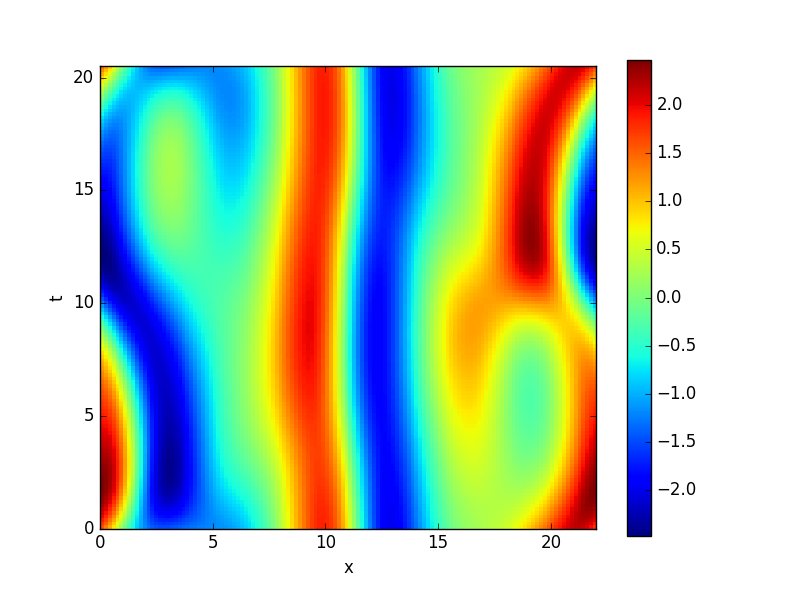
\includegraphics[width=\textwidth,height=.32\textheight]{MNGspacetimeinit1}
\end{minipage}
\begin{minipage}[height=.32\textheight]{.45\textwidth}
\centering \small{\texttt{(b)}}
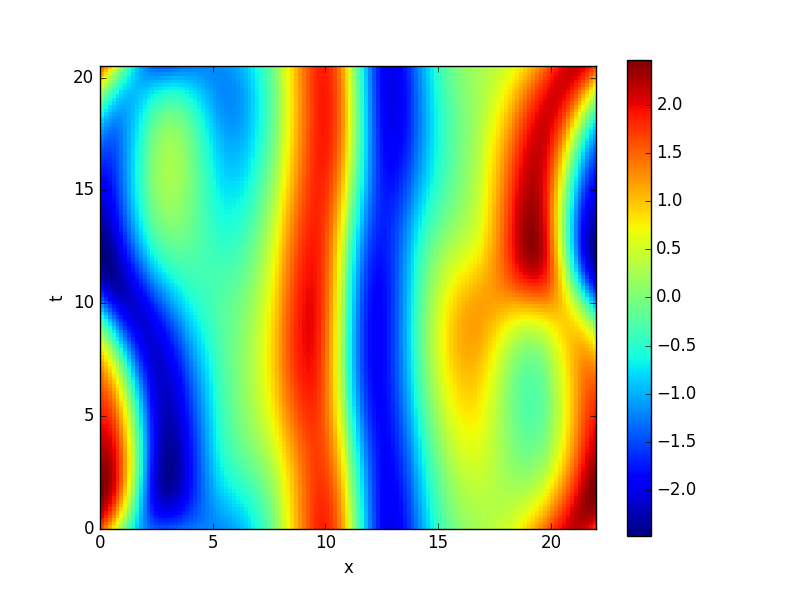
\includegraphics[width=\textwidth,height=.32\textheight]{MNGspacetimefinal1}
\end{minipage}
\caption{ \label{fig:MNGspacetime11}
(a) Initial condition of the 32-by-32 space-by-time discretization of \PPO{10.2}:
$(L_0,\period{0}) = (L_0, 2\period{p_0})= (22,20.5057459345)$.
(b) Resulting spatiotemporal fixed point
$(L_p,2\period{p}) =  (22.0000104401, 20.5057499188)$
}
\end{figure}

\begin{figure}
\begin{minipage}[height=.32\textheight]{.45\textwidth}
\centering \small{\texttt{(a)}}
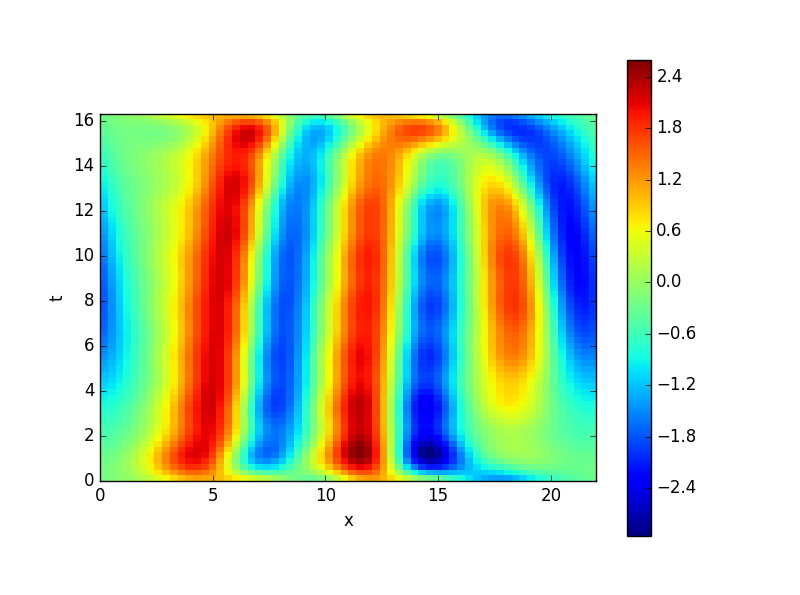
\includegraphics[width=\textwidth,height=.32\textheight]{MNGvndspaceinit2}
\end{minipage}
\\
\begin{minipage}[height=.32\textheight]{.45\textwidth}
\centering \small{\texttt{(b)}}
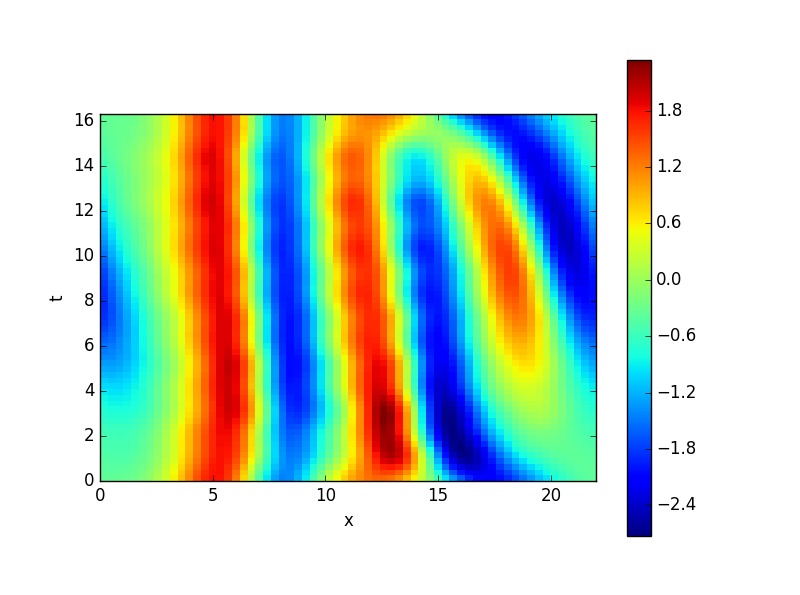
\includegraphics[width=\textwidth,height=.32\textheight]{MNGvndtimefinal2}
\end{minipage}
\begin{minipage}[height=.32\textheight]{.45\textwidth}
\centering \small{\texttt{(c)}}
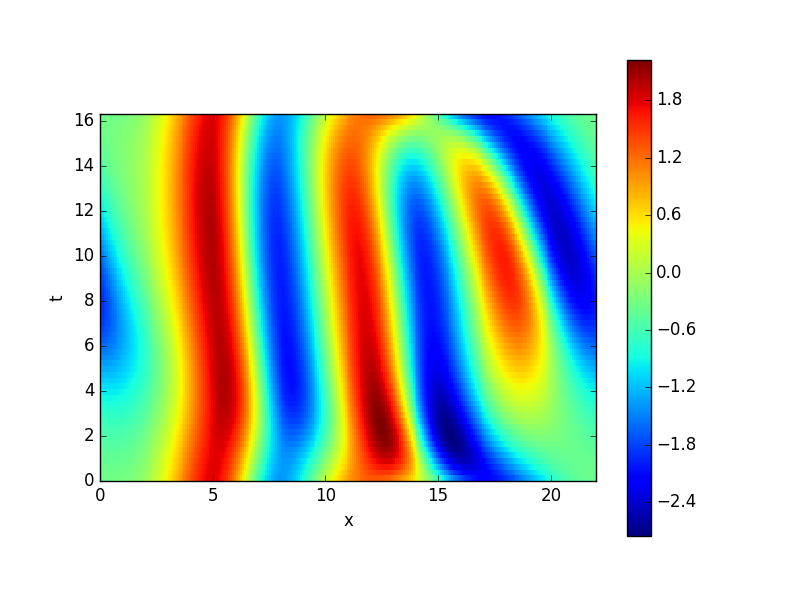
\includegraphics[width=\textwidth,height=.32\textheight]{MNGvndspacefinal2L}
\end{minipage}
\caption{ \label{fig:MNGspaceandtime1}
(a) Initial condition of the 16-by-16 space-by-time discretization of
\RPO{16.31}. $L_0 = 22$.
(b) Resulting periodic orbit after variational {\descent} in time $L =
22, T = 15.7444884386$,
(c) resulting periodic orbit after variational {\descent} in space.
%%%lost the number for final spatial size will need to run code again.
}
\end{figure}

As a means of cross-checking results I wrote variational {\descent} code for time, debugged, and got it working. It follows the "direct-matrix" approach
that I have been finding useful.
The velocity equation takes the form
\beq \label{e-MNGkstimeDM}
v = Q_1 \cdot \Fu - Q_2 \cdot F \cdot ((F^{-1}\Fu) \star (F^{-1}\Fu))
\eeq
and the stability matrix is therefore
\beq
A = Q_1 - 2 * Q_2 * \cdot F \cdot diag(F^{-1}\Fu) \cdot F^{-1}
\eeq

\reffig{fig:MNGspaceandtime1} is a comparison between resulting orbits from both space and time variational {\descent}.
The general structure of the resulting orbit is preserved even though the periods are quite different. At first I believed that
these were supporting evidence that something is going right but now I am confused. The spatial domain resulting from the \emph{spatial}
{\descent} is largely unchanged, meaning that the orbit that results should be a unique solution with a unique period; but the \emph{time}
variational {\descent} changes the period somewhat drastically, and because the spatial domain size is fixed this might mean that I am
finding the same solution but this is contradictory because the periods are so different. Also good evidence that there is something wrong is that
the \emph{time} {\descent} is taking a \rpo\ initial condition and seemingly changing it into a periodic orbit? I don't know what
to think of it but I am glad that I rewrote the time {\descent} code as it'll be a good stepping stone into whether or not I need to rewrite the equations
in a symmetry reduced form in order to find {\rpo}s or not. I think that's where I'm headed at least.




By taking a recurrence from ergodic trajectories using a crude Poincar\'e section
formulation, and then using convolution with a Gaussian mollifier yields bad
spatiotemporal results. Due to the discrepancy between the few steps of convergence
it takes for known orbits and the complete lack of convergence for the few new orbits
tried it seems to indicate that either the initial Newton residual for convergence has
to be smaller than what I am starting with. $10^{-3}$ seems to be the maximum
for the initial residual value.
In short, it could be the size of the discretizations limiting convergence, generating
initial conditions in a bad way, or just Newton's method failing.

The \ppo\ specific formulation of most of the differentiation operators
and Fourier transform operators are finished. They are hard to explain
due to their very specific natures but I will try my best.

The current formulation for the spatiotemporal mapping for {\ppo}s
is

\beq \label{e-spatiotempPPO}
W \cdot \Fu + Q_1 \cdot \Fu + F \cdot ((F^{-1} \cdot \Fu) \ast (F_x^{-1} \cdot Q_2 \cdot F_t^{-1} \cdot \Fu)) = 0
\eeq

The spatiotemporal Fourier transform operators are produced by taking the non-commutative products
$F = F_t \cdot F_x$ and $F^{-1} = F_x^{-1} \cdot F_t^{-1}$. Note, they are only non-commutative due
to the very specific way in which non-zero spatiotemporal Fourier coefficients are produced in order
to have a numerically advantageous linear system to solve later down the line. One could, if so desired,
flip the order but the matrices would have to change accordingly.

In their current formulation, $F_x$ is the operator the enacts the spatial Fourier transform on the
configuration space spatiotemporal velocity field defined on a M-by-N discretization. The output
of the transformation is a vector consisting of the real and imaginary components of the spatial
Fourier spectrum for positive half of the spectrum, i.e. $\tilde{u}_k$ for $k = 1,2,3, \ldots N/2-1$,
as this is all the information required to reproduce the original spatiotemporal velocity field. The
$k=0$ mode is dropped due to Galilean invariance and the $k = N/2$ mode is dropped from requiring it
to be zero because we begin with a real-valued field.

The operator that performs a forwards Fourier transform in time, $F_t$ is an unusual operator that
will not work outside of the context of {\ppo}s . It produces the nonzero portion of the spatiotemporal
Fourier spectrum which consists of the odd modes in time for the real components of the spatial spectrum
and the even modes in time for the imaginary component of the spatial spectrum. Another way of describing
this is to say it really is performing two different Fourier transforms in time at once, one which keeps the odd
numbered time modes $\Fu_{k,\ell}, \mbox{where,} \ell = odd$ and one which produces the even numbered time
modes $\Fu_{k,\ell}, \mbox{where,} \ell = even$. The benefit of such a transformation is that we can solve
for only the variables that are relevant to the spatiotemporal fixed point system of equations, and the
dimensionality of the problem is halved.

The one tricky part of the new formulation is that the nonlinear term needs to be evaluated in a specific
manner given these new definitions. It's a subtle difference, described by evaluating the nonlinear term
with either $-\frac{1}{2}(u^2)_\conf$ or $-u u_\conf$. Although they represent the same quantity, the order
in which the operations are applied when using my specific selection of spatiotemporal Fourier coefficients
(i.e. choice of Fourier transform operators) will drastically change to result.

The quantity $-u u_\conf$ will produce the correct values while $-\frac{1}{2}(u^2)_\conf$ will produce a vector
of zeros. This has to do with the underlying spectrum and the computation of the nonlinear term pseudospectrally,
something that is hard for me to quantify without sounding convoluted but here is my best attempt. The reflection
symmetry will make it such that the real component of the spatial spectrum always goes through one period, while
the imaginary part of the spatial spectrum goes through two. If you are using a very specific formulation of
the Fourier transform (like I am) and you attempt to square the function before applying the spectral differentiation
operator,you will get a null vector because the product lies in the same subspace, but the square alone does not.

Now that the core code is written it should be noted that there are still many improvements that can
be made to the actual numerical scheme solving the equations. I am using the Python equivalent of LAPACK's linear
solver which is ok to work with with small discretizations.

Also to be noted, normally for Newton-Krylov methods, the action of the \jacobianM\ on elements of the tangent
space in a dynamical system is approximated by finite-differences of integrated equations. I might be
able to just employ Python's (SciPy's technically) GMRES implementation because I am explicitly forming the
stability matrix of the spatiotemporal fixed points. (There is no mapping forward in "time" so I am trying to avoid
using the term `\jacobianM'. I believe this is consistent with other \HREF{Chaosbook.org} notation but I will probably
be told otherwise).

Still writing code to find spatiotemporal fixed points of {\rpo}s that are parameterized
in time with the dynamical time instead of rescaled in-slice time. It's taking some time
given the current formulation of my codes because the equations that primary equations
that govern the in-slice velocity and stability matrices are hard to reconcile with the
direct-matrix formulation using a vector that tracks the spatiotemporal Fourier coefficients.

I ran into this problem a little before and ended up switching to the in-slice time formulation
because it was easier to implement; the key problem is that the inner products in the equations
cannot mix time-dependent quantities, such as the velocity and group tangents. This can be
alleviated by converting the $M*N$ dimensional spatiotemporal velocity vector into a $M-by-N$ matrix
such that the matrix-vector product of this "velocity matrix" and group tangent template which
defines the first Fourier mode slice $V \cdot t'$ equals a vector whose elements each represent an
inner product. It isn't the prettiest method but it gets the job done.



After more debugging I realize I was just expecting the initial condition generation
code to know whether something was a \ppo\ without programming it that way,
made corrections to the recurrence plot formulation to be computed with
$||\sigma u(t + \tau) - u(t)||$ and for the best guess to be plucked from that array of
values. This, in conjuction with modifying the Poincar\'e condition, will hopefully
only allow {\ppo}s to be found if that is what is desired. The modification of the
Poincar\'e condition is that the Poincar\'e section is now determined by the reflection
of the initial starting point, meaning that the procedure should now pick out the prime
period of any \ppo. The entire periodic orbit will then be produced by applying the
reflection symmetry on the prime period, glueing them together, and smoothing out
any high Fourier mode components that exist.

Got the R\"ossler code working to find equilibria; I can already see in this
simple system why a hybrid Newton-adjoint code is worthwhile, as even for this system
as the residual of one of the fixed points is reduced to within machine precision
while the other only goes to $10^{-8}$ in the same amount of fictitious time;


Implemented a spatiotemporal way of producing initial conditions for the R\"ossler system that utilizes
random number generation and products of the Fourier spectrum with Gaussian distributions. With this I can produce
(non-physical) initial conditions whose spatial complexity varies with the standard deviation
of the gaussian distribution. The general idea is that because we have time periodicity for the spatiotemporal
fixed points, as long as the Fourier (power) spectrum (in time) exhibits a geometric convergence to zero it
should converge towards a spatiotemporal fixed point when utilizing the adjoint methods employed.

The equations that I will describe are the spatiotemporal mapping described by discretizing the \KSe\ in
space and time, and then taking a spacetime Fourier transform that transforms the equations into a set
of nonlinear algebraic equations dependent on the spatiotemporal Fourier coefficients.
If I may be so bold as to begin with the equations written in terms of the Galerkin truncation in space and
time of spatiotemporal Fourier coefficients;

I will denote the components of the mapping $F$ which is dependent on all of the spatiotemporal Fourier coefficients $\Fu_{k,l}$
as such:

\beq \label{e-MNGspattemp}
F(\Fu)_{k,\ell} = (i\omega_\ell -q_k^2 +q_k^4 )\Fu_{k,l} + iq_k/2 \sum_{\prime{k},\prime{\ell}} \Fu_{k-\prime{k},\ell-\prime{\ell}} \Fu_{k,\ell}
\eeq

Personally, I find it much easier in avoiding to mistakes to represent this mapping as matrix representations acting upon a spatiotemporal vector,
AND I have elected to represent the spatiotemporal Fourier coefficients by their real valued representations. The reason behind the real-valued
representations is that there are some underlying conjugacy conditions due to symmetries in the spectrum
such that the number of independent variables is far fewer than the total number of complex spatiotemporal Fourier coefficients, and I find
it easier to deal with these conditions in a real-valued representation. If one doesn't handle these conjugacy conditions then the linear
system of equations we desire to solve later will be singular and yield nonsense. In the words of Viswanath, "Determining the exact dimension
of the vector $x$ can be a little tricky because one needs to eliminate
Fourier coefficients that are conjugates of certain others and so on"\rf{Visw08}, I elect for simplicity which will hopefully be agreed upon after reading this.

Due to the ordering of the Fourier coefficients previously \emph{not} elucidated upon, the structure of the spatiotemporal vector will cycle through
all values of spatial index $k$ before changing the temporal index $\ell$. In a visual example this corresponds to
\beq \label{e-MNGstvec}
\transp{[\Fu_{k,l}]} = \transp{[\Fu_{k,0}, \Fu_{k,1}, \ldots, \Fu_{k,M/2}]}
\eeq
This notation can be somewhat confusing,especially more so when discrete symmetries
are taken into account, but hopefully I can clarify in this manner: When I take a spatial Fourier transform
with real-valued notation, then only half of the spectrum $k > 0$ is independent information. This is because the configuration
space field is real valued, the spatial Fourier coefficients
take follow the conjugacy rule $u_k(t) = u_{-k}^*(t)$.

In order to have a real valued representation these must be split between real and
imaginary components, i.e. $u_k(t) = a_k(t) + i b_k(t)$.

Now, $a_k(t)$ and $b_k(t)$ again constitute real valued series in time, so one follows the same procedure but in time (different ordering).

By doing so we can formulate differential operators to act on vectors with such an ordering,
in an absence of knowledge about naming conventions,

I will denote $W$ as the differential operator that, using spectral
differentiation, produces the time derivative of our spatiotemporal field; equivalent to multiplication of
the respective spatiotemporal Fourier coefficients
by $i \omega_\ell$.

$Q_1$ will denote
the differential operator that produces the second and fourth spatial derivatives, equivalent
to multiplication by $-q_k^2 +q_k^4$

$Q_2$ will denote
the differential operator that produces the first spatial derivative divided by two, equivalent
to multiplication by $i q_k / 2$.

$\mathcal{F}$ and $\mathcal{F}^{-1}$ will denote the matrix representations
of forward, and backward spatiotemporal Fourier transforms.

As to the explicit structures of these matrix representations, look further down.
With these definitions the nonlinear algebraic equation takes the following form.

\beq
F(\Fu) = ( W + Q_1) \Fu + Q_2 \mathcal{F} ((\mathcal{F}^{-1} \Fu)*(\mathcal{F}^{-1} \Fu)) \mbox{where} \, * \equiv \mbox{entrywise multiplication}
\eeq

For starters let us survey what linearizing about the trivial equilibrium $\Fu{k,\ell}=0$ yields.

\beq \label{e-MNGstlintriv}
\frac{\partial F(\Fu)}{\partial \Fu}|_{\Fu = 0} = W + Q_1 \equiv L
\eeq

The structure of $L = W + Q_1$ is copies of $-q_k^2 +q_k^4$ along the diagonal, and $-w_k$ on a
superdiagonal and $w_k$ on a subdiagonal.

The structure of $L$ is such that the multipliers take
the form $\Lambda_{k,l} = (-q_k^2 +q_k^4) \pm i w_\ell$, in addition to two marginal modes which should
are due to temporal and spatial translations. These two modes are dealt with by imposing two constraints.



In this regard. If we apply a perturbation to the trivial equilibrium, $\delta \Fu = \delta \Fu_{k=4,\ell=0}$
whose $L^2$ norm is reasonably small, then the spatiotemporal mapping yields $F(\delta \Fu) = (-q_4^2 +q_4^4)\delta \Fu_{k=4,\ell=0}$

This is relatively interesting as the spectrum of \reffig{fig:MNGsttrivmult}, if I am interpreting it correctly, seems to indicate
that somehow time is related to rotation while space is related to stretching.

A similar spectrum can be obtained for spatiotemporal fixed points
corresponding to {\ppo}s, except with some modulation in space due to the
nonlinear contribution. for {\rpo}s most of the structure is seemingly
lost. I don't have any results from antisymmetric orbits $\in \bbU^+$ but
I will try to provide an example of each tomorrow.

The general description of the adjoint method is that we are stepping
in fictitious time determined by $-\transp{J(\Fu)} F(\Fu)$ as this ensures that
the cost functional will monotonically decrease to $0$. The description of the improvements
can be summed up by the following.

The linear component of the spatiotemporal mapping, and thus the contribution
to the \jacobianM\ is dominated by the contribution by the Laplacian and
Laplacian squared terms of the \KSe. The way it presents itself in the
contribution to the \jacobianM\ of the mapping is to have a dominant
diagonal. This is one of the instances where use of a diagonal (Jacobi)
preconditioner is motivated.



\begin{figure}
\begin{minipage}[height=.32\textheight]{.45\textwidth}
\centering \small{\texttt{(a)}}
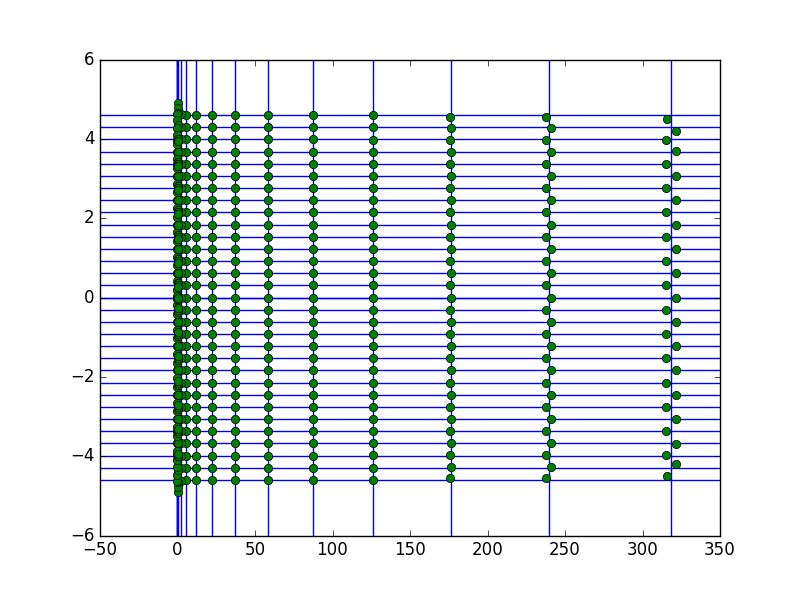
\includegraphics[width=\textwidth,height=.32\textheight]{MNGppo1_spectrum}
\end{minipage}
\\
\begin{minipage}[height=.32\textheight]{.45\textwidth}
\centering \small{\texttt{(b)}}
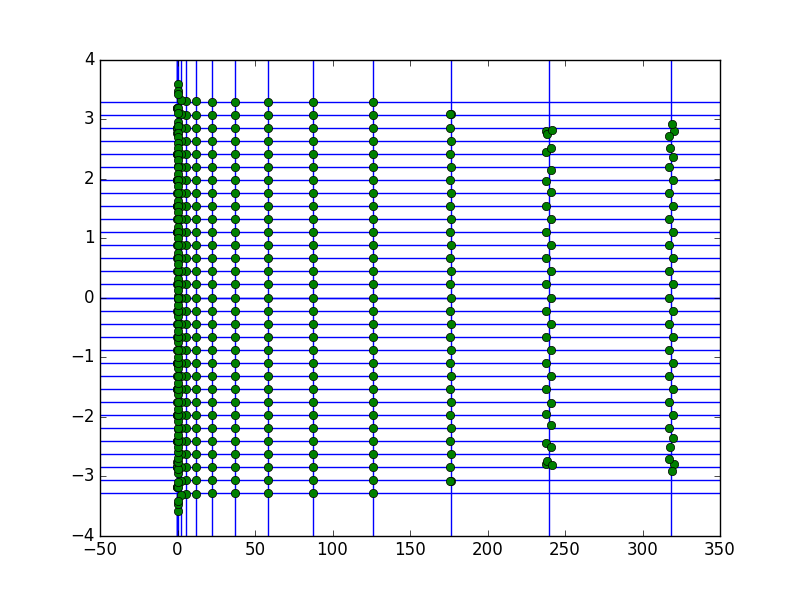
\includegraphics[width=\textwidth,height=.32\textheight]{MNGppo2_spectrum}
\end{minipage}
\begin{minipage}[height=.32\textheight]{.45\textwidth}
\centering \small{\texttt{(c)}}
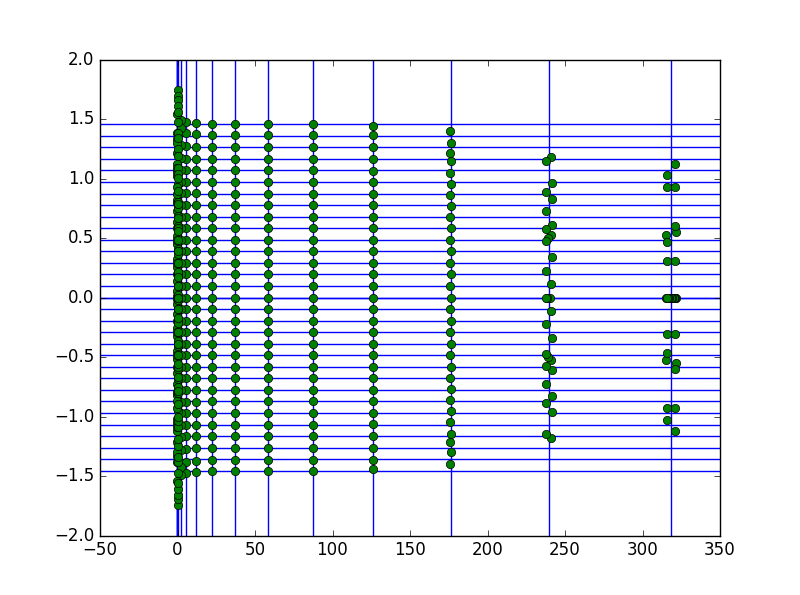
\includegraphics[width=\textwidth,height=.32\textheight]{MNGppo3_spectrum}
\end{minipage}
\caption{ \label{fig:MNGppospacetimespec}
(a) Spatiotemporal multiplier spectrum for \PPO{10.2},
(b) Spatiotemporal multiplier spectrum for \PPO{14.3},
(c) Spatiotemporal multiplier spectrum for \PPO{32.3}.
Intersections between horizontal and vertical lines indicate where the
multipliers would be for the $u(\conf,\zeit)=0$.
In other words, changes from this grid indicate
differences between the linearized spatiotemporal spectrum and the full
spatiotemporal spectrum. All three solutions converged to within machine
precision when defined on a 32-by-32 spacetime grid; Fourier calculations
done with $15 \times 31$ spatiotemporal Fourier coefficients.
}
\end{figure}

In reference to the post of {\bf 2017-03-14},
%\phantomsection\label{2017-03-14MNG} % refer to it by
on page~\pageref{2017-03-14MNG}
in \refchap{chap:dailyBlog}~{\em
Space-time, blogged} I would argue that what I have done is quite similar to
L{\'o}pez \etal\rf{lop05rel}.

By using the spacetime Fourier-Fourier basis representation of the spatiotemporal field with
Galerkin truncations in space and time
\beq   \label{eqn:mng_am_ansatz_ks}
    \am{m}(t)  =  \sum_{n \in \integers} \akj \e^{\ii \omegaj t} \, ,
\eeq
The nonlinear algebraic equations in this basis are \refeq{e-FksSpattemp}.
I will restate the equations here
for completeness and comparison to L{\'o}pez \etal\rf{lop05rel}.
In the spacetime Fourier-Fourier basis, the \KSe\ takes
the form,
\beq
\left[ \ii \omegaj - ( \wavek^2 - \wavek^4 ) \right] \akj
+ \frac{ \ii \wavek }{2} \!\sum_{k'} \sum_{j'}\!\!
\akj a_{k-k',j-j'}
    = 0
\,.
\ee{FkSpattemp}
while in L{\'o}pez \etal\rf{lop05rel}, with the ansatz for {\rpo}
solutions \refeq{eqn:am_ansatz} the \cGL\ take the form
\bea
\ii \left( \frac{2 \pi n}{T} - \frac{\varphi}{T} - m \frac{S}{T} \right)\,\akj
    &=&
    R \akj  - m^2 (1+\ii \nu)\akj
    \label{eqn:spacetime_lop05rel}\\
    - (1+ \ii \mu)\sum_{m'}
      \sum_{n'} a_{k_1,j_1} a_{k_2,j_2} a_{k_3,j_3}^{*}
\,,
\nnu
\eea
where $m_1+m_2-m_3 = m'$ and $n_1+n_2-n_3 = n'$.

The differences between our methods arise when setting up the equation as a root
solving procedure. In L{\'o}pez \etal\rf{lop05rel} the numerics is handled by solving for the
roots of the function $F(\akj ,\varphi , S, T) = 0$ where $F$ is the function described
by \refeq{eqn:spacetime_lop05rel} if one moved all of the terms to one side of the equation.

In my current procedure, I solve
\refeq{e-FksSpattemp}, % PC: Matt had here {eqn:FksSpattemp}
or for comparison,
$F(\akj, T, L) = 0$, where $T,L$ are in the factors $\omegaj,\wavek$ respectively.

I do not explicitly include variables that control the spatial translations of the system and,
up until now, have elected to search for {\rpo} solutions pertaining to
\refeq{e-FksSpattemp} % PC: Matt had here {eqn:FksSpattemp}
by finding them in the first Fourier mode slice. Part of the reason of this was I didn't
understand the reasoning behind parameterizing the spatial translations by $\zeit$ by means
of the factor in the ansatz $\e^{-\ii \wavek \frac{S}{T}t}$. I thought the shift factor
had to be explicitly calculated by the coordinates, and not assumed through this type of time
dependence.

My comments of
{\bf 2017-11-02} on page~\pageref{2017-11-02MNG}
were mainly predicated by the fact that once we find these roots, I don't think
we can apply the same type of reasoning as Politi and Torcini\rf{PolTor92b} as
they aren't truly fixed points of a fictitious dynamical system, like so,
$F(\akj, T, L) = {\akj, T, L}$. But rather, like I have already
described, they are the roots of a system of nonlinear algebraic equations,
$F(\akj, T, L) = 0$.

If I am so inclined to change how I search for relative periodic orbits in the same manner as
L{\'o}pez \etal\rf{lop05rel} I believe all I would have to actually implement is this $\e^{-\ii \wavek \frac{S}{T}t}$
factor in my ansatz, such that the new equations for solutions with $\SOn{2}$ symmetry would be,
\beq
\left[ \ii \omegaj - m \frac{S}{T} - ( \wavek^2 - \wavek^4 ) \right] \akj
+ \frac{ \ii \wavek }{2} \!\sum_{n'} \sum_{m'}\!\!
\akj a_{k-k',j-j'}
    = 0
\,.
\label{eqn:FksSpattemp_rel}
\eeq
such that the spatiotemporal solutions would now be roots of the nonlinear system of equations,
$F(\akj, S, T, L) = 0$

Working my way towards an implementation of the reposed spatiotemporal problem that
involves inverting a differential operator (the sum of second and fourth spatial derivative operators)
defined by equation \refeq{eqn:MNGspacetime_reform}, restated here for completeness.

\bea
G(\Fu, T, L) &\equiv& D_X^{-1}(D_t \Fu + D_x F (F^{-1} \Fu)^2 ) - \Fu = 0
    \continue
D_X &\equiv& D_{xx} - D_{xxxx}
\eea

When treated as the true fixed point problem, the action of $G(x)$ on doubly periodic solutions
is an involution, meaning that points get mapped to themselves. Although this last statement
is obvious, I am stating it because it demonstrates the (what I consider to be)
unnatural behavior of the alternative
problem, where, no matter where you are in this spatiotemporal {\statesp}, every doubly
periodic solution gets mapped to zero under the action of $F$. I believe this to be unnatural
because if you're looking at the linearization of this spatiotemporal function $F$ you are
looking at the linear neighborhood at a point in spatiotemporal {\statesp} that is necessarily
far away from the original doubly periodic solution. Also, the other part I find unnatural about
this is that because every doubly periodic solution is being mapped to zero, all of the solutions
are in a sense being identified to one another no matter where they really exist. There is probably
a smarter and or more precise way of rephrasing that last sentence but its the best I could come up with.

On the other hand, this is also well motivated in a numerical sense because the reformulation
inverts an operator who is comprised of numbers ranging from order unity to numbers orders of magnitude
larger. This is poor for iterative methods unless one introduces a preconditioning, because these large
diagonal elements will a large range of eigenvalues. The reason this is poor, for say, Newton-Krylov method
is that for an example when there is one dominant eigenvalue, the power iteration that produces
the Krylov subspace, $\mathcal{K}_n = {b, Ab, A^2 b, \dots}$ will tend to converge to the most dominant
eigenvector, and hence its known that such methods work best when the eigenvalues are clustered near unity.

So effectively, by reposing the problem by inverting the diagonal operator I am effectively rescaling
space as one might do by either preconditioning or by defining a Sobolev norm to use instead of the
usual $L_2$ norm.

I added code that works in physical space after computing derivatives in Fourier-Fourier space,
the main incentive was to try and see if Jianke Yang's claim that it's better to work in the
"PDE framework" agrees with me. Sadly it doesn't seem to be the case for me. I didn't do things
exactly like he did, and I guess what I in fact implemented could be described by saying
"everything is the same except the linear system of equations that I need to solve are in terms of
the physical velocity field $u$ and not its spatiotemporal Fourier components."



Realized that reformulating the {\rpo} spatiotemporal code to encode the \SOn{2} shift with a parameter is a larger
undertaking then I thought, due to all of the different dependencies of the code I have currently; The general
idea is that the shift can be parameterized by time, although I still feel like this is somehow only incorporating
a specific time of translation; In other words I can't shake the feeling that

The general idea is to produce an ansatz for the relation between endpoints (initial point and the
endpoint i.e. point after one prime period) on a {\rpo} in such a fashion (described in terms of
spatial Fourier modes to make the representation of the translation easier),
\beq \label{e-MNG_rpo_st_ansatz}
\Fu_k(0) =e^{i k S t/T_p}\Fu_k(T) \, ,
\eeq
where the spatial drift, shift, etc. is parameterized by time and a shift parameter $S$. The
form of the rescaled spatiotemporal mapping would then take the following form.
\bea \label{e-MNG_rpo_spacetime_reform}
x &=& (\Fu, T, L, S)
    \continue
G(x) &\equiv& D_X^{-1}((D_t + D_S) \Fu + D_x F (F^{-1} \Fu)^2 ) - \Fu
    \continue
D_X &\equiv& D_{xx} - D_{xxxx}
\eea
where $x$ is a vector representing all of the varying quantities $(\Fu , T_p, L, S)$, and $D_S$
is an operator representing the time derivative of the exponential prefactor in \refeq{e-MNG_rpo_st_ansatz}

Tried to trawl {\statesp} for initial conditions for my spatiotemporal code and realized that
it ran really slowly for small step sizes (large number of steps). Figured out how to speed
it up by rewriting some key parts of the close recurrence calculations; realized I was sloppy
when it came with the actual optimization previously. Essentially by unrolling some 'for'-loops
and rewriting some key portions I was able to dramatically speed it up. 